\documentclass{article}
\textheight=25.5cm
\textwidth=16.0cm
\oddsidemargin=-0.5cm
\topmargin=-3.0cm
\usepackage[pdftex]{graphicx}
\usepackage[utf8]{inputenc}
\usepackage[spanish]{babel}
\title{Taller \# 5 de F\'isica 2\\ FISI 1028, Semestre 2014 - 10}
\author{Profesor: Jaime Forero}
\date{Viernes, 21 de Febrero, 2014}
\begin{document}
\maketitle
\thispagestyle{empty}

\noindent
Este taller debe ser preprarado y discutido para la clase
complementaria de la semana del 24 de Febrero del 2014. 

\noindent
{\bf Importante}:
\begin{itemize}

\item
Las respuestas a los cuatro primeros ejercicios se deben entregar al comenzar la
clase complementaria. 
\item 
Los \'ultimos tres ejercicios son para participaci\'on en clase y entrega
durante la complementaria. {\bf{Tambi\'en}} los deben llevar casi
terminados. En la complementaria (adem\'as de resolver dudas) se
calificar\'a la participaci\'on al tratar de resolver estos ejercicios
finales en el tablero. La idea es poder terminar los  detalles de esos
\'ultimos puntos para entregarlos al final de la complementaria.
\end{itemize}

\begin{enumerate}

\item
Ejercicio 21.5 (Atracci\'on entre dos personas).

\item
Ejercicio 21.10 (Masa vs. carga)

\item
Ejercicio 21.11 (Un experimento en el espacio).

\item
Ejercicio 21.24 (Tres cargas en equilibrio)


\item 
Suponga que se logra separar un cent\'imetro c\'ubico de agua en sus
cargas elementales de signos contrarios. Suponga ahora que se logran
separar estos dos conjuntos de cargas elementales entre s\'i por
$100$km. ¿Con qué fuerza (en Newtons) se atraen?

\item
Tres cargas positivas, $q_1$, $q_2$ y $q_3$ est\'an unidas entre ellas
por dos hilos. La longitud de cada hilo es $l$. Encuentre la fuerza de
tensi\'on de cada hilo.

\item
\label{exo:hex}
Siete cargas id\'enticas $q$ est\'an unidas la unas a las otras por
cuerdas el\'asticas como se muestra en la Figura \ref{fig:hex}. La
distancia entre dos cargas vecinas es $l$. Encuentre la fuerza de
tensión de todas las cuerdas. 
\end{enumerate}


\begin{figure}[h!]
\begin{center}
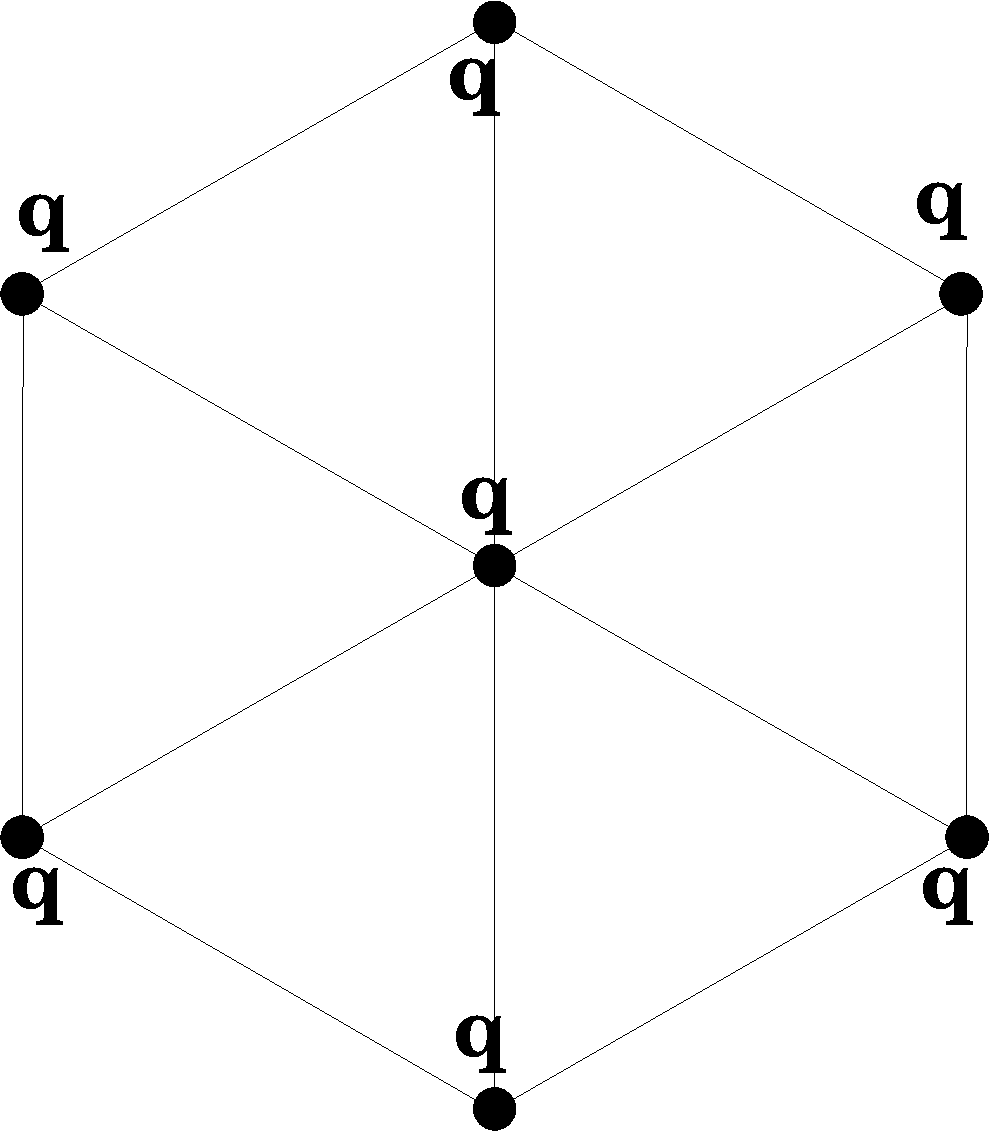
\includegraphics[scale=0.20]{figs/hexagono.pdf}
\end{center}
\caption{Diagrama para el problema \ref{exo:hex}}
\label{fig:hex}
\end{figure}


\end{document}
